\exercice{Automatismes, connaître son cours (15 minutes)}\label{exo:auto}\points{10}
\medskip

\numeroQuestion
Relier chaque grandeur à son symbole et à l'unité associée.
\points{3}

\begin{center}    
  \begin{tblr}{
    width=\textwidth,
    colspec = {Q[wd=0.25\linewidth, l] Q[wd=0.15\linewidth, l] r Q[wd=0.1\linewidth, c] Q[wd=0.15\linewidth, l] r Q[wd=0.1\linewidth, c]},
    row{1} = {couleurPrim!20, c}
  }
  %% ALIGNER PLUS DE GRANDEUR 
    \textbf{Grandeur}      & & & \textbf{Symbole} & & & \textbf{Unité} \\
    Concentration massique & \pointCyan & \pointCyan & $n$   & \pointCyan & \pointCyan &  \unit{\mole\per\litre} \\
    Quantité de matière    & \pointCyan & \pointCyan & \variationSujet{$C_m$}{$\lambda$} & \pointCyan & \pointCyan &  \unit{\kelvin} \\
    Concentration molaire  & \pointCyan & \pointCyan & \variationSujet{$\lambda$}{$C_m$}   & \pointCyan & \pointCyan &  \unit{\g\per\mole} \\
    Masse molaire          & \pointCyan & \pointCyan & $T$   & \pointCyan & \pointCyan & \variationSujet{\unit{\mole}}{\unit{\g\per\litre}} \\
    Température            & \pointCyan & \pointCyan & $C$   & \pointCyan & \pointCyan & \unit{\m} \\
    Longueur d'onde        & \pointCyan & \pointCyan & $M$   & \pointCyan & \pointCyan & \variationSujet{\unit{\g\per\litre}}{\unit{\mole}}
  \end{tblr}
\end{center}


% \numeroQuestion Donner le nom de ces deux ions \points{1}
% \begin{center}  
%   \oxonium : \texteTrou[0.1]{ion oxonium} \qq{}
%   et \hydroxyde : \texteTrou[0.1]{ion hydroxyde}
% \end{center}

% \question{
%   Définir \variationSujet{un acide}{une base} d'après Br\o{}nsted. \points{1}
% }{
%   C'est une espèce chimique qui peut libérer des ions \chemfig{H^+}.
%   \points{1}
% }[2]
\question{
  Définir un \variationSujet{réducteur}{oxydant}.\points{1}
}{}[1]

\numeroQuestion
Indiquer sur l'échelle pH ci-dessous où se trouve les solutions acides, les solution basiques et les solutions neutres.
Puis placer sur cette échelle pH les solutions suivantes : \points{2}
\begin{tableau}{|c |c |c |c |c |c |}
  Solution & \variationSujet{Acide chlorhydrique}{Acide éthanoïque} & Acide sulfurique & \variationSujet{Soude}{Savon} & Eau & Eau de mer \\
  pH       & \variationSujet{\num{3,1}}{\num{4,2}} & \num{1,0} & \variationSujet{\num{13,9}}{\num{8,9}} & \num{7,0} & \num{8,1} 
\end{tableau}

\pasCorrection{\vspace*{30pt}}
\begin{center}
  \begin{tikzpicture}
    \tikzVecteur (-0.75, 0) (15.5, 0) {pH}
    \foreach \i in {0,1,...,14} \draw (\i,0.1)--(\i,-0.1) node[below]{\i};
  \end{tikzpicture}
\end{center}

\question{
  Pour les \variationSujet{myopes}{hypermétropes}, les lunettes correctrices comportent des verres plus \variationSujet{épais}{fins} sur les côtés qu'au centre.
  Indiquer le type de lentille mince utilisées pour les verres des lunettes.
  Justifier.\points{1,5}
}{}[2]

\numeroQuestion
Sur le spectre électromagnétique suivant, indiquer où se trouve le domaine infrarouge.
\points{1}
\begin{center}
  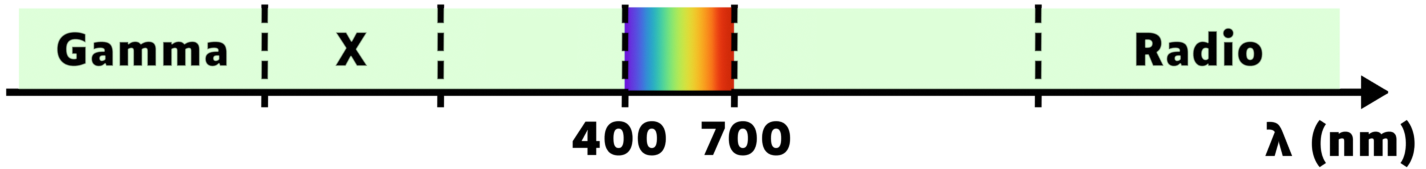
\includegraphics[width = \linewidth]{images/spectre_EM_a_completer}
\end{center}

\question{
  Expliquer comment doit être la couche externe des éléments chimiques pour être stable en formant des molécules.
  \points{1,5}
}{}[2]
